\documentclass[11pt,letterpaper,english]{article}

\usepackage[margin=1.0in]{geometry}
\usepackage{helvetica}
\usepackage[table]{xcolor}
\usepackage{graphicx}

\title{Effects of Economic Relase Data on Market Health Indicators}
\author{Ian Clark}
\date{}

\begin{document}
\maketitle

\section{The ISM Manufacturing Index}
With a consensus range from 53.5 to 56.5 and a mean consensus of 55, the data for the ISM Manufacturing Index was released lower than predicted at 53.5. 

\subsection{Affects Upon the Market}
Affects upon the S\&P 500 were questionable at best, as the general economic climate was already slipping into turmoil because of European news concerning the European Central Bank and Greece's new Finance Minister Yanis Varoufakis.

\section{The Employment Situation}
The employment situation data has all-around been fantastic, with consistently high revisions ranging from November's astounding revisions in Non-farm month-to-month Payroll to February's release data. Considering the trend (please see below data), further positive revisions seem both feasible and plausible.

\begin{center}
    \begin{tabular}{| c | c | c | c |}
    \hline
    Month       & Original (1000s) & Revised (1000s) & Difference (1000s) \\ \hline
    November    & 353 & 423 & \cellcolor{green}{+70} \\ \hline
    December    & 252 & 329 & \cellcolor{green}{+77} \\ \hline
    January     & 321 & 353 & \cellcolor{green}{+32} \\ \hline
    February    & 257 & \cellcolor{black}{} & \cellcolor{black}{} \\ \hline
    \end{tabular}
\end{center}

Moreover, the Unemployment Level (the u3) has risen (employment has increased) from 5.6\% to 5.7\%, albeit this seems to indicate the economy is in such a promising position that many previously discouraged workers have opted to return to the job search, thus creating a slight convergence between the u3 and u6 employment rates. 
Contributing to this, we saw a rise from 62.7\% labor force participation to 62.9\% This statistic, however, is not as impressive, as the trend has been for labor force participation to remain near 62.9\%, as seen below:

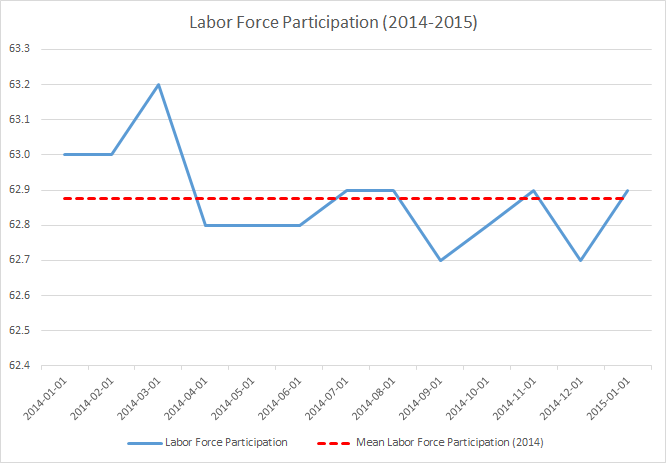
\includegraphics[scale=0.85]{LaborForceParticipation.png}

\subsection{Affects Upon the Market}

\end{document}